\documentclass{article}

\usepackage{arxiv}

\usepackage[utf8]{inputenc} % allow utf-8 input
\usepackage[T1]{fontenc}    % use 8-bit T1 fonts
\usepackage{lmodern}        % https://github.com/rstudio/rticles/issues/343
\usepackage{hyperref}       % hyperlinks
\usepackage{url}            % simple URL typesetting
\usepackage{booktabs}       % professional-quality tables
\usepackage{amsfonts}       % blackboard math symbols
\usepackage{nicefrac}       % compact symbols for 1/2, etc.
\usepackage{microtype}      % microtypography
\usepackage{graphicx}

\title{Determinação da extensão espacial da paisagem local}

\author{
    Danilo Pereira Mori
   \\
    LET - IBUSP \\
   \\
  \texttt{} \\
  }

% Pandoc syntax highlighting
\usepackage{color}
\usepackage{fancyvrb}
\newcommand{\VerbBar}{|}
\newcommand{\VERB}{\Verb[commandchars=\\\{\}]}
\DefineVerbatimEnvironment{Highlighting}{Verbatim}{commandchars=\\\{\}}
% Add ',fontsize=\small' for more characters per line
\usepackage{framed}
\definecolor{shadecolor}{RGB}{248,248,248}
\newenvironment{Shaded}{\begin{snugshade}}{\end{snugshade}}
\newcommand{\AlertTok}[1]{\textcolor[rgb]{0.94,0.16,0.16}{#1}}
\newcommand{\AnnotationTok}[1]{\textcolor[rgb]{0.56,0.35,0.01}{\textbf{\textit{#1}}}}
\newcommand{\AttributeTok}[1]{\textcolor[rgb]{0.77,0.63,0.00}{#1}}
\newcommand{\BaseNTok}[1]{\textcolor[rgb]{0.00,0.00,0.81}{#1}}
\newcommand{\BuiltInTok}[1]{#1}
\newcommand{\CharTok}[1]{\textcolor[rgb]{0.31,0.60,0.02}{#1}}
\newcommand{\CommentTok}[1]{\textcolor[rgb]{0.56,0.35,0.01}{\textit{#1}}}
\newcommand{\CommentVarTok}[1]{\textcolor[rgb]{0.56,0.35,0.01}{\textbf{\textit{#1}}}}
\newcommand{\ConstantTok}[1]{\textcolor[rgb]{0.00,0.00,0.00}{#1}}
\newcommand{\ControlFlowTok}[1]{\textcolor[rgb]{0.13,0.29,0.53}{\textbf{#1}}}
\newcommand{\DataTypeTok}[1]{\textcolor[rgb]{0.13,0.29,0.53}{#1}}
\newcommand{\DecValTok}[1]{\textcolor[rgb]{0.00,0.00,0.81}{#1}}
\newcommand{\DocumentationTok}[1]{\textcolor[rgb]{0.56,0.35,0.01}{\textbf{\textit{#1}}}}
\newcommand{\ErrorTok}[1]{\textcolor[rgb]{0.64,0.00,0.00}{\textbf{#1}}}
\newcommand{\ExtensionTok}[1]{#1}
\newcommand{\FloatTok}[1]{\textcolor[rgb]{0.00,0.00,0.81}{#1}}
\newcommand{\FunctionTok}[1]{\textcolor[rgb]{0.00,0.00,0.00}{#1}}
\newcommand{\ImportTok}[1]{#1}
\newcommand{\InformationTok}[1]{\textcolor[rgb]{0.56,0.35,0.01}{\textbf{\textit{#1}}}}
\newcommand{\KeywordTok}[1]{\textcolor[rgb]{0.13,0.29,0.53}{\textbf{#1}}}
\newcommand{\NormalTok}[1]{#1}
\newcommand{\OperatorTok}[1]{\textcolor[rgb]{0.81,0.36,0.00}{\textbf{#1}}}
\newcommand{\OtherTok}[1]{\textcolor[rgb]{0.56,0.35,0.01}{#1}}
\newcommand{\PreprocessorTok}[1]{\textcolor[rgb]{0.56,0.35,0.01}{\textit{#1}}}
\newcommand{\RegionMarkerTok}[1]{#1}
\newcommand{\SpecialCharTok}[1]{\textcolor[rgb]{0.00,0.00,0.00}{#1}}
\newcommand{\SpecialStringTok}[1]{\textcolor[rgb]{0.31,0.60,0.02}{#1}}
\newcommand{\StringTok}[1]{\textcolor[rgb]{0.31,0.60,0.02}{#1}}
\newcommand{\VariableTok}[1]{\textcolor[rgb]{0.00,0.00,0.00}{#1}}
\newcommand{\VerbatimStringTok}[1]{\textcolor[rgb]{0.31,0.60,0.02}{#1}}
\newcommand{\WarningTok}[1]{\textcolor[rgb]{0.56,0.35,0.01}{\textbf{\textit{#1}}}}

% tightlist command for lists without linebreak
\providecommand{\tightlist}{%
  \setlength{\itemsep}{0pt}\setlength{\parskip}{0pt}}



\begin{document}
\maketitle


\begin{abstract}

\end{abstract}


\hypertarget{introduuxe7uxe3o}{%
\section{Introdução}\label{introduuxe7uxe3o}}

Aqui determino a extensão espacial da paisagem local ao redor da parcela
amostrada usando a análise de escala de efeito (REF). A análise de
escala de efeito se baseia em determinar a extensão espacial da paisagem
local que maximiza o peso de evidência da regressão entre o número de
espécies na parcela e a proporção de cobertura vegetal dos 109 sítios de
amostragens selecionados na base TreeCo. Primeiro calculamos a proporção
de cobertura vegetal para paisagens locais quadradas em que variamos a
extensão espacial da paisagem. Fizemos uma sequência de extensões
espaciais somando 0.12 km no lado da paisagem. A menor paisagem
apresentou 0.3km de lado, aproximadamente o lado da maior parcela caso
ela fosse quadrada (área de 10.24 ha, lado de 0.32 km). E a maior
extensão espacial apresentou 11 km de lado. Ao todo foram 108 extensões
espaciais. Então é calculado o peso de evidência da regressão para cada
extensão espacial. Aquela extensão que atribuir maior peso de evidência
será selecionada para determinar a extensão espacial da paisagem local.

\hypertarget{calcular-a-proporuxe7uxe3o-de-cobertura-vegetal-para-cada-extensuxe3o-espacial}{%
\section{calcular a proporção de cobertura vegetal para cada extensão
espacial}\label{calcular-a-proporuxe7uxe3o-de-cobertura-vegetal-para-cada-extensuxe3o-espacial}}

\begin{Shaded}
\begin{Highlighting}[]
\NormalTok{f\_pEscalas }\OtherTok{\textless{}{-}} \ControlFlowTok{function}\NormalTok{(df)\{}
\NormalTok{  df\_p }\OtherTok{\textless{}{-}} \FunctionTok{data.frame}\NormalTok{(}\AttributeTok{p =} \ConstantTok{NA}\NormalTok{, }\AttributeTok{lado\_km =} \ConstantTok{NA}\NormalTok{)}
\NormalTok{  m\_full }\OtherTok{\textless{}{-}} \FunctionTok{raster}\NormalTok{(df}\SpecialCharTok{$}\NormalTok{tif.path) }\SpecialCharTok{|\textgreater{}}\NormalTok{ raster}\SpecialCharTok{::}\FunctionTok{as.matrix}\NormalTok{()}
\NormalTok{  i\_centro }\OtherTok{\textless{}{-}} \FunctionTok{nrow}\NormalTok{(m\_full)}\SpecialCharTok{/}\DecValTok{2}
\NormalTok{  v\_last\_i }\OtherTok{\textless{}{-}}\NormalTok{ (i\_centro}\DecValTok{{-}5}\SpecialCharTok{+}\DecValTok{2}\NormalTok{)}\SpecialCharTok{/}\DecValTok{2}
  \ControlFlowTok{for}\NormalTok{(i }\ControlFlowTok{in} \DecValTok{1}\SpecialCharTok{:}\NormalTok{v\_last\_i)\{}
\NormalTok{    v\_add }\OtherTok{\textless{}{-}} \DecValTok{5}\SpecialCharTok{+}\DecValTok{2}\SpecialCharTok{*}\NormalTok{(i}\DecValTok{{-}1}\NormalTok{)}
\NormalTok{    m\_i }\OtherTok{\textless{}{-}}\NormalTok{ m\_full[(i\_centro}\SpecialCharTok{+}\DecValTok{1}\SpecialCharTok{{-}}\NormalTok{v\_add)}\SpecialCharTok{:}\NormalTok{(i\_centro}\SpecialCharTok{+}\NormalTok{v\_add),}
\NormalTok{                  (i\_centro}\SpecialCharTok{+}\DecValTok{1}\SpecialCharTok{{-}}\NormalTok{v\_add)}\SpecialCharTok{:}\NormalTok{(i\_centro}\SpecialCharTok{+}\NormalTok{v\_add)]}
\NormalTok{    df\_p[i,] }\OtherTok{\textless{}{-}} \FunctionTok{c}\NormalTok{(}\FunctionTok{length}\NormalTok{(m\_i[m\_i}\SpecialCharTok{==}\DecValTok{1}\NormalTok{])}\SpecialCharTok{/}\FunctionTok{length}\NormalTok{(m\_i),}
                  \FunctionTok{nrow}\NormalTok{(m\_i) }\SpecialCharTok{*} \DecValTok{30}\SpecialCharTok{/}\DecValTok{1000}\NormalTok{)}
\NormalTok{  \}}
\NormalTok{  df\_p}\SpecialCharTok{$}\NormalTok{SiteCode }\OtherTok{\textless{}{-}}\NormalTok{ df}\SpecialCharTok{$}\NormalTok{SiteCode}
  \FunctionTok{return}\NormalTok{(df\_p)}
\NormalTok{\}}
\FunctionTok{registerDoMC}\NormalTok{(}\DecValTok{3}\NormalTok{)}
\NormalTok{df\_pEscalas }\OtherTok{\textless{}{-}} \FunctionTok{adply}\NormalTok{(df\_dados,}\DecValTok{1}\NormalTok{,f\_pEscalas,}\AttributeTok{.id =} \StringTok{"SiteCode"}\NormalTok{,}\AttributeTok{.parallel =} \ConstantTok{TRUE}\NormalTok{)}
\FunctionTok{write\_csv}\NormalTok{(}\AttributeTok{x =} \FunctionTok{select}\NormalTok{(df\_pEscalas,Ntotal,S\_obs,p}\SpecialCharTok{:}\NormalTok{SiteCode),}
          \AttributeTok{file =} \StringTok{"./dados/csv/df\_EscalaEfeito.csv"}\NormalTok{)}
\end{Highlighting}
\end{Shaded}

\hypertarget{ajustar-os-modelos-para-um-mesmo-lado_km}{%
\section{Ajustar os modelos para um mesmo
lado\_km}\label{ajustar-os-modelos-para-um-mesmo-lado_km}}

S\_obs = riqueza observada na parcela;

p = proporção de cobertura vegetal;

Ntotal = número de indivíduos vivos na parcela;

\begin{Shaded}
\begin{Highlighting}[]
\NormalTok{df\_se }\OtherTok{\textless{}{-}} \FunctionTok{read\_csv}\NormalTok{(}\StringTok{"./dados/csv/df\_EscalaEfeito.csv"}\NormalTok{)}
\NormalTok{f\_glm.nb }\OtherTok{\textless{}{-}} \ControlFlowTok{function}\NormalTok{(data\_)\{}
\NormalTok{  md\_ }\OtherTok{\textless{}{-}}\NormalTok{ MASS}\SpecialCharTok{::}\FunctionTok{glm.nb}\NormalTok{(S\_obs }\SpecialCharTok{\textasciitilde{}}\NormalTok{ p }\SpecialCharTok{+} \FunctionTok{I}\NormalTok{(p}\SpecialCharTok{\^{}}\DecValTok{2}\NormalTok{) }\SpecialCharTok{+} \FunctionTok{I}\NormalTok{(p}\SpecialCharTok{\^{}}\DecValTok{3}\NormalTok{) }\SpecialCharTok{+} \FunctionTok{offset}\NormalTok{(}\FunctionTok{log}\NormalTok{(Ntotal)), }\AttributeTok{data =}\NormalTok{ data\_)}
\NormalTok{\}}
\FunctionTok{registerDoMC}\NormalTok{(}\DecValTok{3}\NormalTok{)}
\NormalTok{l\_md }\OtherTok{\textless{}{-}} \FunctionTok{dlply}\NormalTok{(df\_se,}\StringTok{"lado\_km"}\NormalTok{,f\_glm.nb,}\AttributeTok{.parallel =} \ConstantTok{TRUE}\NormalTok{)}
\end{Highlighting}
\end{Shaded}

\hypertarget{calcular-o-peso-de-eviduxeancia-por-lado-da-paisagem-local-km}{%
\section{Calcular o peso de evidência por lado da paisagem local
(km)}\label{calcular-o-peso-de-eviduxeancia-por-lado-da-paisagem-local-km}}

\begin{Shaded}
\begin{Highlighting}[]
\NormalTok{df\_averageSE }\OtherTok{\textless{}{-}} \FunctionTok{print}\NormalTok{(}\FunctionTok{AICctab}\NormalTok{(l\_md,}\AttributeTok{weights=}\ConstantTok{TRUE}\NormalTok{),}\AttributeTok{min.weight=}\DecValTok{10}\SpecialCharTok{\^{}}\NormalTok{(}\SpecialCharTok{{-}}\DecValTok{10}\NormalTok{)) }\SpecialCharTok{\%\textgreater{}\%} 
  \FunctionTok{as.data.frame}\NormalTok{()}
\NormalTok{df\_averageSE}\SpecialCharTok{$}\NormalTok{lado\_km }\OtherTok{\textless{}{-}} \FunctionTok{row.names}\NormalTok{(df\_averageSE) }\SpecialCharTok{\%\textgreater{}\%} \FunctionTok{as.numeric}\NormalTok{()}
\NormalTok{df\_averageSE}\SpecialCharTok{$}\NormalTok{weight }\OtherTok{\textless{}{-}} \FunctionTok{as.numeric}\NormalTok{(}\FunctionTok{as.character}\NormalTok{(df\_averageSE}\SpecialCharTok{$}\NormalTok{weight))}
\NormalTok{df\_averageSE}\SpecialCharTok{$}\NormalTok{dAICc }\OtherTok{\textless{}{-}} \FunctionTok{as.numeric}\NormalTok{(}\FunctionTok{as.character}\NormalTok{(df\_averageSE}\SpecialCharTok{$}\NormalTok{dAICc))}
\end{Highlighting}
\end{Shaded}

\hypertarget{selecionar-o-lado-da-paisagem-local-que-atribuiu-maior-peso-de-eviduxeancia}{%
\section{Selecionar o lado da paisagem local que atribuiu maior peso de
evidência}\label{selecionar-o-lado-da-paisagem-local-que-atribuiu-maior-peso-de-eviduxeancia}}

\begin{Shaded}
\begin{Highlighting}[]
\NormalTok{df\_averageSE }\SpecialCharTok{|\textgreater{}} \FunctionTok{filter}\NormalTok{(weight}\SpecialCharTok{==}\FunctionTok{max}\NormalTok{(df\_averageSE}\SpecialCharTok{$}\NormalTok{weight))}
\end{Highlighting}
\end{Shaded}

\begin{verbatim}
##       dAICc df  weight lado_km
## 22.26     0  5 0.03989   22.26
\end{verbatim}

\hypertarget{avaliauxe7uxe3o}{%
\section{Avaliação}\label{avaliauxe7uxe3o}}

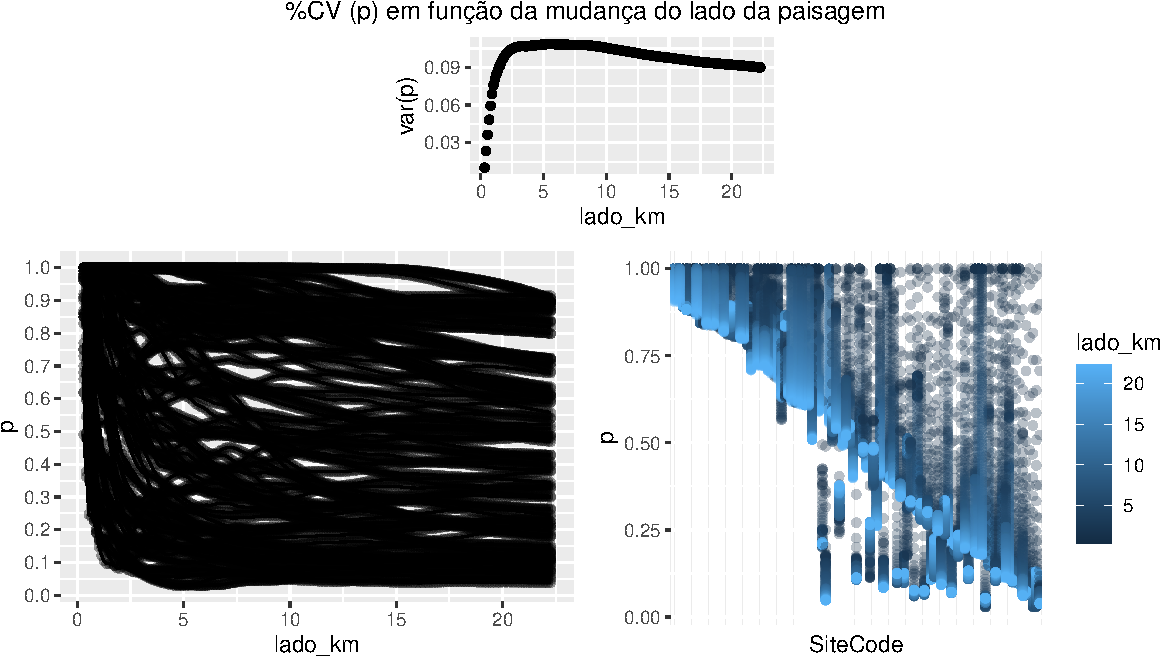
\includegraphics{EfeitoEscala_files/figure-latex/figura p por lado da paisagem-1.pdf}

\textbf{Figura 1} Proporção de cobertura vegetal (\%CV) em relação ao
lado da paisagem (lado\_km). SiteCode = código da paisagem.

\bibliographystyle{unsrt}
\bibliography{references.bib}


\end{document}
